% ------------------------------------------------------------------------------
% TYPO3 Version 9.4 - What's New (German Version)
%
% @license	Creative Commons BY-NC-SA 3.0
% @link		https://typo3.org/help/documentation/whats-new/
% @language	German
% ------------------------------------------------------------------------------

\section{Backend User Interface}
\begin{frame}[fragile]
	\frametitle{Backend User Interface}

	\begin{center}\huge{Kapitel 1:}\end{center}
	\begin{center}\huge{\color{typo3darkgrey}\textbf{Backend User Interface}}\end{center}

\end{frame}

% ------------------------------------------------------------------------------
% Admin Panel (1)

\begin{frame}[fragile]
	\frametitle{Backend User Interface}
	\framesubtitle{Admin Panel (1)}

    Das Admin Panel hat eine komplette Überarbeitung hinsichtlich des Designs und des zugrunde liegenden
    Kodes.
	\newline\newline
	Das Admin Panel wird im Frontend am Ende der Seite angezeigt.
	Die auf der rechten Seite ermöglicht Integratoren und Editoren die Aktivierung 
	und Deaktivierung des Admin Panels. Der aktuelle Status zeigt den Status \textit{enabled} an.

	\begin{figure}
		
\includegraphics[width=0.90\linewidth]{BackendUserInterface/AdminPanelEnabled.png}
	\end{figure}

\end{frame}

% ------------------------------------------------------------------------------
% Admin Panel (2)

\begin{frame}[fragile]
	\frametitle{Backend User Interface}
	\framesubtitle{Admin Panel (2)}

	Der folgende Screenshot zeigt TypoScript-Optionen.

	\begin{figure}
		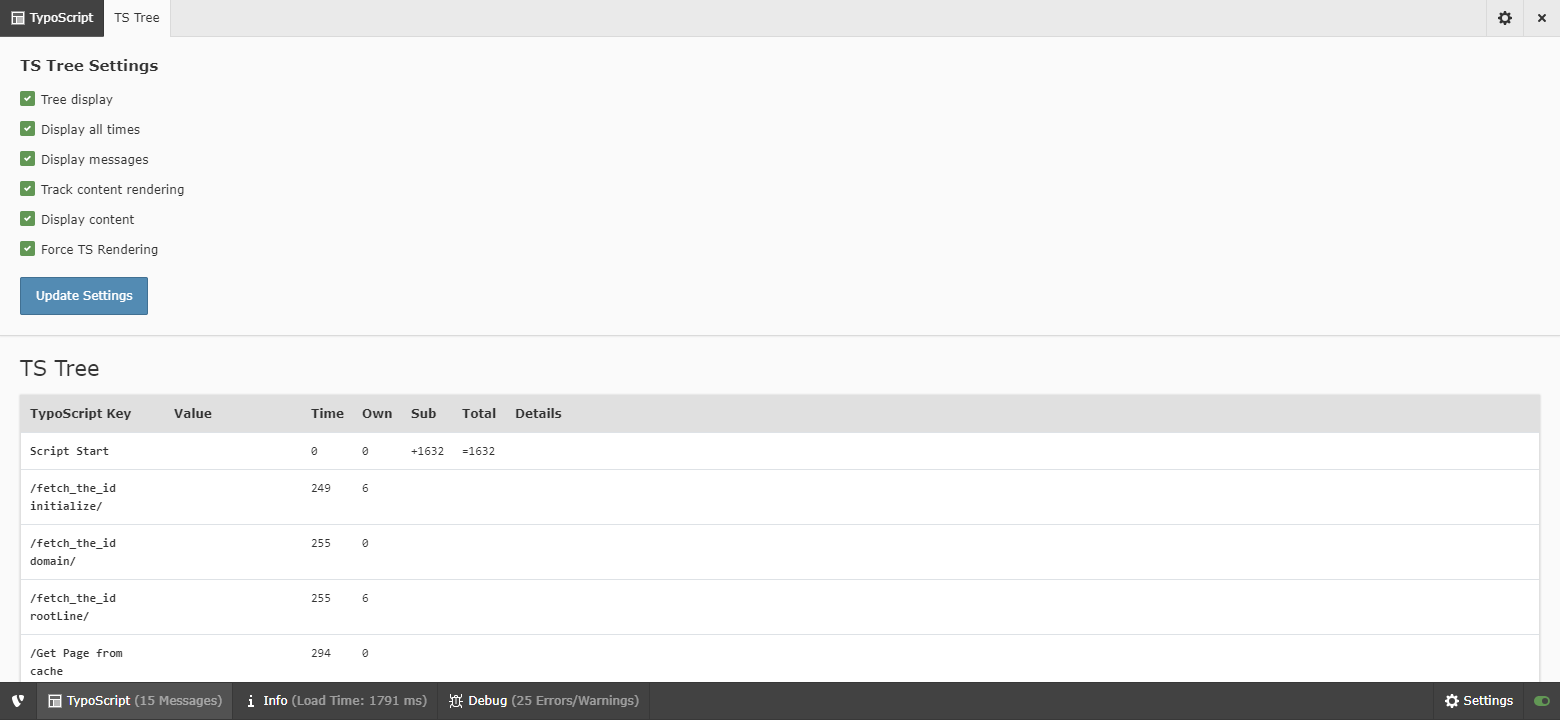
\includegraphics[width=0.90\linewidth]{BackendUserInterface/AdminPanelTypoScript.png}
	\end{figure}

\end{frame}

% ------------------------------------------------------------------------------
% Admin Panel (3)

\begin{frame}[fragile]
	\frametitle{Backend User Interface}
	\framesubtitle{Admin Panel (3)}

	Der folgende Screenshot zeigt Konfigurationsoptionen ("Settings").

	\begin{figure}
		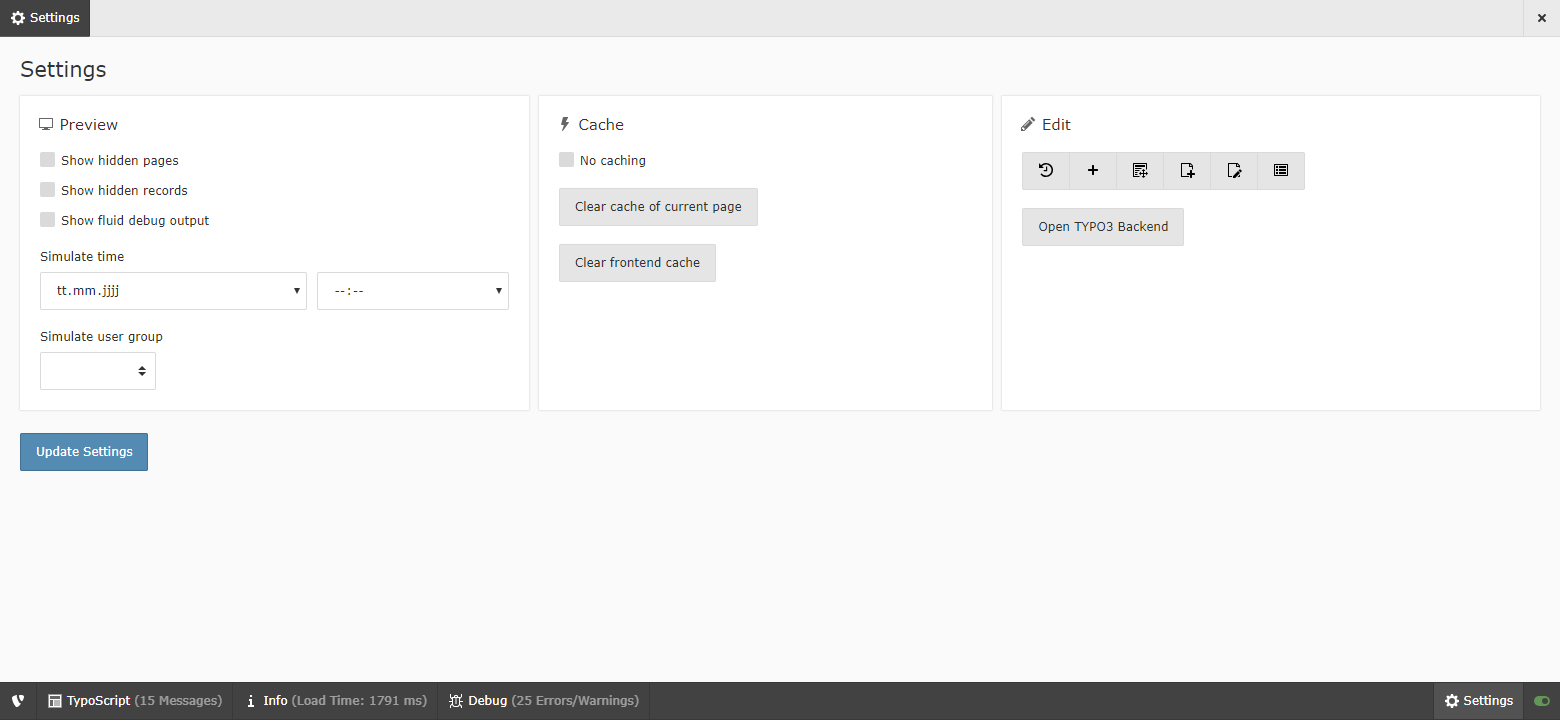
\includegraphics[width=0.90\linewidth]{BackendUserInterface/AdminPanelSettings.png}
	\end{figure}

\end{frame}

% ------------------------------------------------------------------------------
% #85398 - EXT:documentation removed

\begin{frame}[fragile]
	\frametitle{Backend User Interface}
	\framesubtitle{Die Extension "Documentation" Removed}

	Das Modul "Documentation" wurde aus dem TYPO3-Backend entfernt.
    Das Modul hatte technische und konzeptionelle Mängel und die Akzeptanz innerhalb der TYPO3 Community  
    war nicht zu hoch.
    \newline
    Die Documentation bleibt unter \href{https://docs.typo3.org}{docs.typo3.org} verfügbar.

	\begin{figure}
		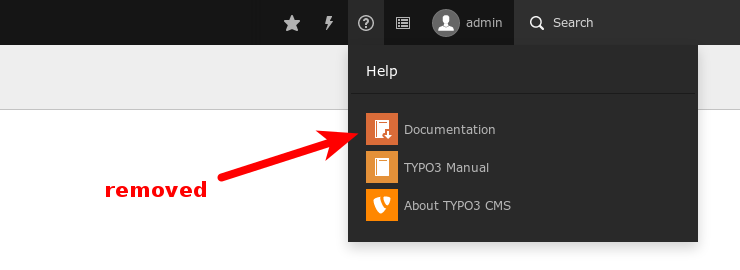
\includegraphics[width=0.70\linewidth]{BackendUserInterface/85398-ExtensionDocumentationRemoved.png}
	\end{figure}

\end{frame}

% ------------------------------------------------------------------------------
% #13265 - Select first element of page tree toolbar on initialization

\begin{frame}[fragile]
	\frametitle{Backend User Interface}
	\framesubtitle{Page Tree Toolbar}

	Das erste Element der Page Tree Toolbar wird nun automatisch ausgewählt.

	\begin{figure}
		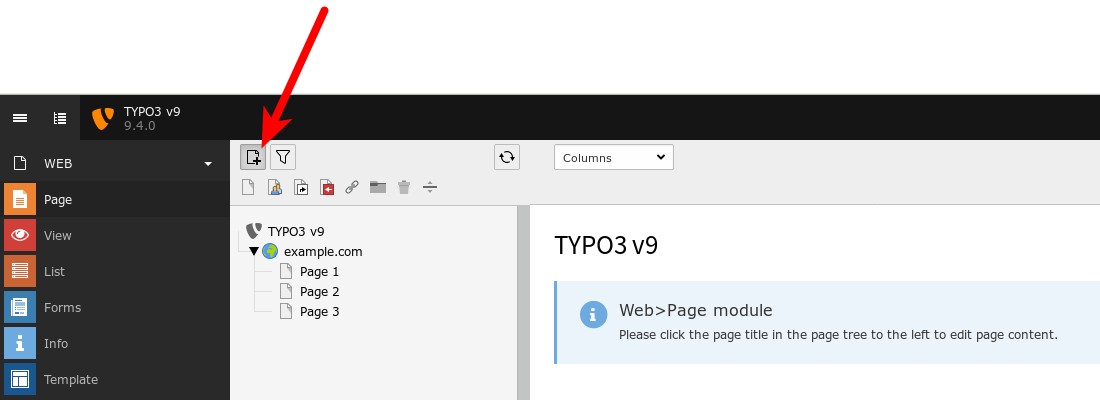
\includegraphics[width=0.90\linewidth]{BackendUserInterface/13265-FirstElementOfPageTree.png}
	\end{figure}

\end{frame}

% ------------------------------------------------------------------------------
% #85313 - Add notes field to pages table

\begin{frame}[fragile]
	\frametitle{Backend User Interface}
	\framesubtitle{Seitennotizen}

	Die Seiten haben nun ein "description" Feld (unter "Notes"). Dieses Feld ermöglicht Benutzer Notizen 
	hinzuzufügen. Andere Backend Benutzer können diese sehen/bearbeiten.

	\begin{figure}
		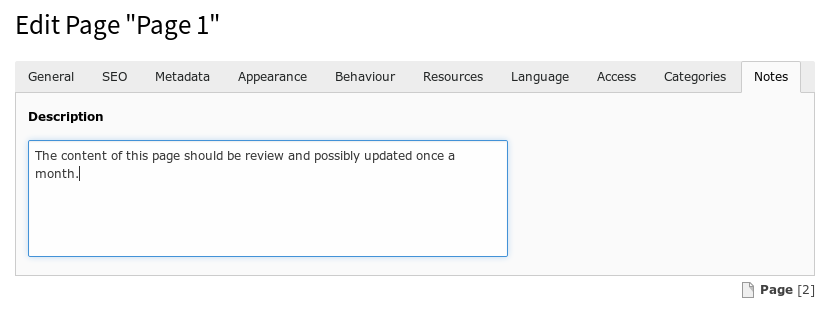
\includegraphics[width=0.90\linewidth]{BackendUserInterface/85313-NotesFieldForPages.png}
	\end{figure}

\end{frame}

% ------------------------------------------------------------------------------
% #xxxxx - Languages Visible in Frontend

\begin{frame}[fragile]
	\frametitle{Backend User Interface}
	\framesubtitle{Nur definierte Sprachen}

	Die Sprachen der Website sind beschränkt im Backend auf die unter
	"Site Management → Site Configuration → Languages" definierten Sprachen. Jede Sprache kann 
	aktiviert/deaktiviert werden.

	\begin{figure}
		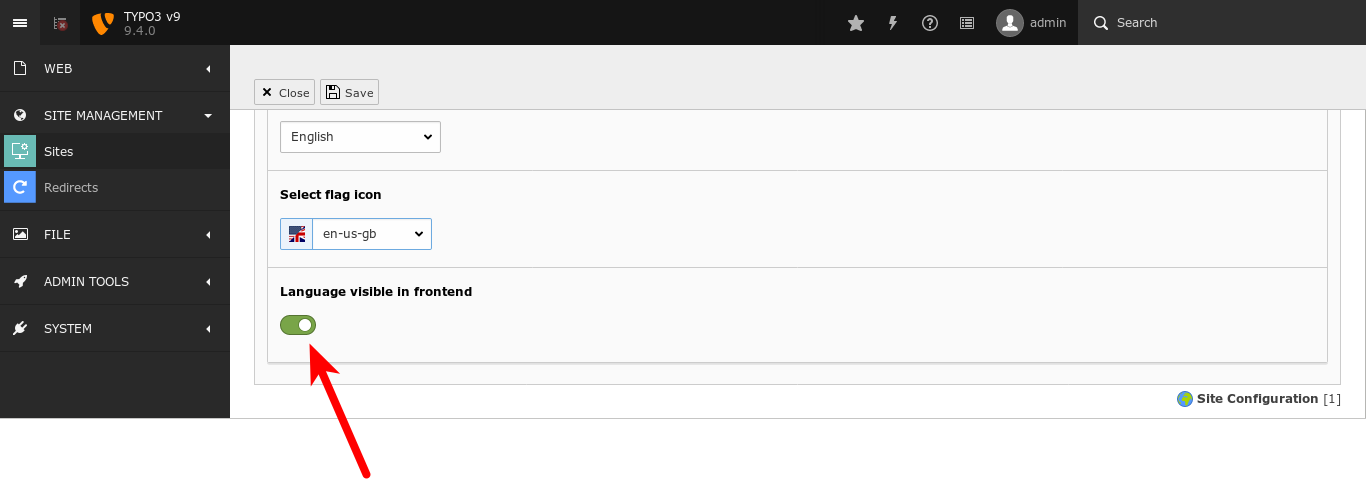
\includegraphics[width=0.90\linewidth]{BackendUserInterface/xxxxx-LanguagesVisibleInFrontend.png}
	\end{figure}

\end{frame}

% ------------------------------------------------------------------------------
% #85691 - Show page path in record info

\begin{frame}[fragile]
	\frametitle{Backend User Interface}
	\framesubtitle{Seitenpfad in Record Info}

	Details zur Referenz von Datensätzen rhalten jetzt den Pfad in der Seitenstruktur.

	\begin{figure}
		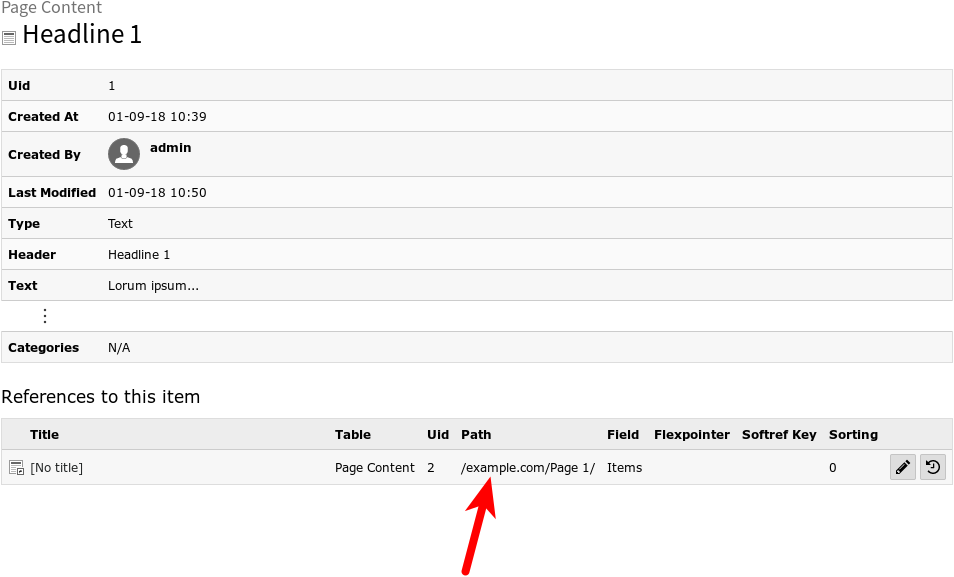
\includegraphics[width=0.70\linewidth]{BackendUserInterface/85691-ShowPagePathInRecordInfo.png}
	\end{figure}

\end{frame}

% ------------------------------------------------------------------------------
% Page-based URL Handling (aka "URL Routing")

\begin{frame}[fragile]
	\frametitle{Änderungen für Integratoren}
	\framesubtitle{Seitenbasierte URL Handling}

 	TYPO3 unterstützt jetzt seitenbasierte URL Handling.

	\begin{figure}
		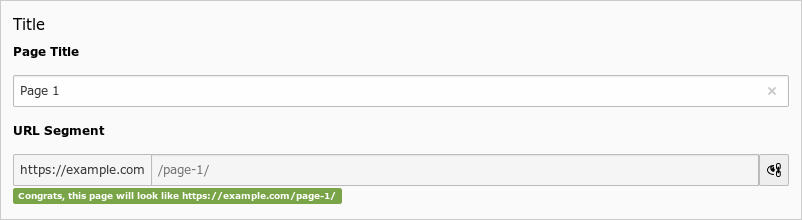
\includegraphics[width=0.90\linewidth]{BackendUserInterface/xxxxx-UrlRouting.png}
	\end{figure}

\end{frame}

% ------------------------------------------------------------------------------
% Modal Windows

% %%%%%%%%%%%%%%%%%%%%%%%%%%%%%%%%%%%%%%%%%%%%%%%%%%%%%%%%%%%%%% %
% Let's do not mention this in v9.4, but in v9.5 (TYPO3 v9 LTS). %
% We aim to achieve that all(!) popups use modal windows by the  %
% release of v9 LTS.                                             %
% %%%%%%%%%%%%%%%%%%%%%%%%%%%%%%%%%%%%%%%%%%%%%%%%%%%%%%%%%%%%%% %

%\begin{frame}[fragile]
%	\frametitle{Backend User Interface}
%	\framesubtitle{Modal Windows}
%
%	Almost all popup windows in the backend of TYPO3 are now "modal windows"
%	rather than small browser windows, which open.
%
%\end{frame}

% ------------------------------------------------------------------------------
